\documentclass{beamer}
\usepackage{amsfonts, amsmath, graphicx, verbatim, graphicx, hyperref,
  color}
\definecolor{UNBlue}{RGB}{91, 146, 229}
\setbeamercolor{structure}{fg=UNBlue}
\newcommand\Fontvi{\fontsize{6.5}{7.2}\selectfont}
\usetheme{Warsaw}


\title{Statistical Standardization\\ of the Supply and Utilization Accounts}
\author{\it Michael C. J. Kao}
\institute{Economic and Social Statistics Division (ESSD)\\ \vspace{0.1in} Food and Agriculture Organization \\ of the United Nations}
\date{\vspace{-0.1in}\today}


\AtBeginSection[]
{
  \begin{frame}<beamer>
    \frametitle{Outline for section \thesection}
    \tableofcontents[currentsection]
  \end{frame}
}

\begin{document}

\frame{
  \titlepage
  \centering
  
\includegraphics[scale = 0.2]{fao_logo.png}
}

\frame{
  \frametitle{Outline}
  \tableofcontents
}


\section{Introduction}

\frame{
  \frametitle{Supply and Utilization Account}

  The Supply and the Utilization Account (SUA) is a detailed
  national account of the supply and utilization of agricultural
  products.

  \vfill
  
  The Food Balance Sheet (FBS) is an aggregated summary of the Supply
  and the Utilization Account.

  \vfill

  Using accounting analogy, SUA is the collection of all trasanction
  took place while FBS is a summary derived from SUA acting like
  financial reports.
  

}


\frame{
  \frametitle{What is standardization}

  Standardization in this context is the procedure of converting
  derived commodity such as wheat flour and bread to a comparable
  standard expression.

  \vfill

  For example, instead of how much wheat flour, bread are consumed
  individually we express it as its wheat equivalent.

  \vfill

  The standardized value enables comparison and also reduce the amount
  of information for comprehension.
  

}


\frame{
  \frametitle{Mapping}

  \vfill
  
  In order to perform standardization, one must specify the
  relationship between the derived commodities and their primary
  commodity. One such instance is the commodity tree shown in the
  following slide.

  \vfill 


}

\frame{

  \begin{figure}
    \centering
    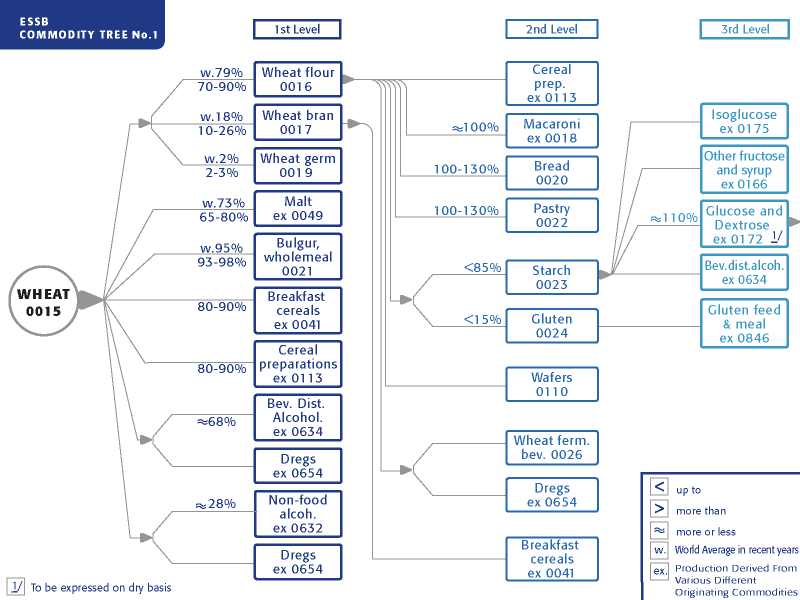
\includegraphics[scale = 0.3]{wheat_commodity_tree.png}
  \end{figure}

}


%% \frame{
%%   \frametitle{}
%%   There are in fact two steps in the standardization.
%%   \begin{itemize}
%%     \setlength{\itemindent}{1in}
%%     \item[Compute the allocation: ] In this step, the import and export
%%   \end{itemize}
%% }


\section{Implementation}
\frame{
  \frametitle{Background}

  The current specification of the commodity tree is technically known
  as a \textbf{rooted tree}.

  \vfill

  A rooted tree is a tree which has a designated vertex known as the
  \textbf{root}. In our case, it is the primary commodity group or the target
  group we would like to standardize to.

  \vfill

  The tree is intuitive but restrictive, in this seminar we would like
  to propose the more general flexible framework of \textbf{graph} for
  standardization.

}

\frame{
  \frametitle{Terminology}
  \begin{itemize}
    \setlength{\itemindent}{1in}
    \item[Vertex: ] A node representing the commodity
    \item[Edge: ] A line connecting the vertex.
    \item[Root: ] A specific designated node.
    \item[Parent: ] The vertex directly above the current vertex.
    \item[Child: ] The vertex directly below the current vertex.
    \item[Leaf: ] A node which has has no child.
  \end{itemize}
  
}

\frame{

  In a rooted tree, a vertex can have and at most one
  \underline{parent}, we would like to relax this and allow multiple
  inputs for each derivative.

  \vfill

  Furthermore, we don't want to fix the selection of the root. We want
  to be flexible and be able to standardize to any equivalence. To
  achieve this, we need the vertex to be able to reach every single
  other vertex.

}

\frame{
  \frametitle{This is more than a figure, its a mathematical model}
  \begin{figure}
    \centering
    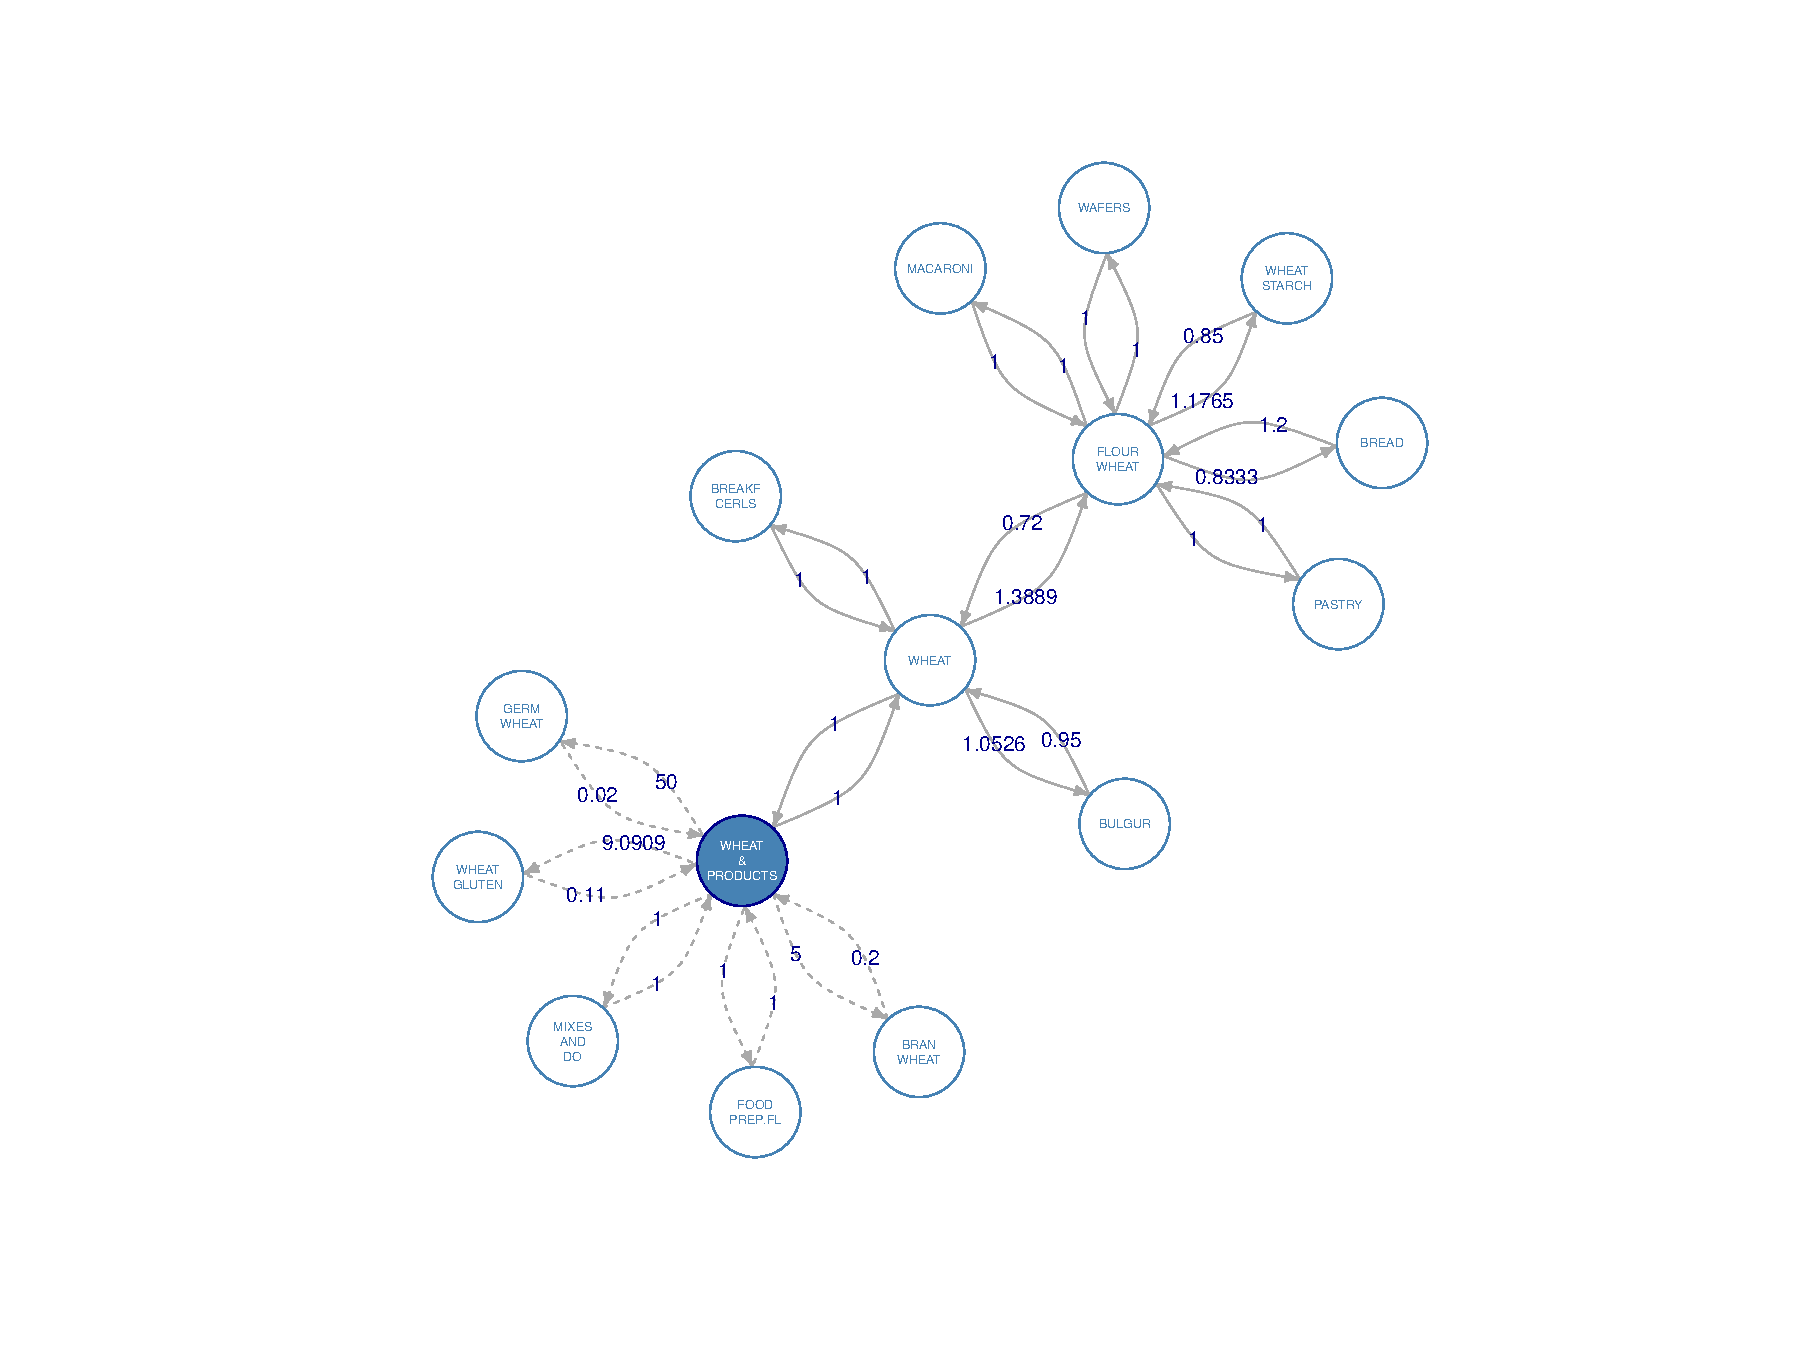
\includegraphics[scale = 0.33]{wheat_network.pdf}
  \end{figure}

}

\frame{
  \frametitle{Difference in Quantity and Calorie Standardization}
  
  %% The item set between quantity and calorie standardization should
  %% be the same. Otherwise, it would not have made any sense. I just
  %% don't see a point of computing a quantity that makes no sense and
  %% inaccurate.

  Quantity Standardization is performed for all element such as
  import/export, waste, seed and other utilization; on the other hand,
  calorie standardization is based solely on food to reflect the
  consumables.
  
  \vfill

  Certain commodity are standardized in calorie but not in
  quantity. For example, only wheat flour are standardized to obtain
  the quantity while wheat germ and bran are not. This is to avoid
  double counting.
 

}

\frame{
  \frametitle{Benefits of a network specification}
  
  \begin{itemize}
    \setlength{\itemindent}{1in}
    \item[Traceability: ] We can see how it is standardized.
    \item[Flexibility: ] It can take every single possible form.
    \item[Simplicity: ] The relationship can be modified easily.
  \end{itemize}
}

\section{Framework for National Accounts}
\subsection{Traditional Accounting Standardization}

\frame{
  \frametitle{Traditional Accounting Standardization}

  Tradtional accounting standardization system assume that everything
  is measured without error, and the standardization procedure is
  merely a matrix arithematic exercise. Furthermore, the frameworkd
  does not capture the error in model based estimation of elements
  such as feed and waste.

  \vfill

  This is both unrealistic in practice and problematic as we
  over-state our confidence about the derived statistic.

}

\subsection{Probabilistic Convolution Standardization}

\frame{ 
  \frametitle{Probabilistic Convolution Standardization of the SUA} 

  To account for the over-simplified scenario of the accounting
  system, we propose to use a statistical framework for
  standardization.

  \vfill

  Quantities can be specified as distribution to reflect uncertainty
  or lack of state of knowledge. 


}

\frame{
  \frametitle{Statistical Standardization of the SUA}

  Take the commodity tree for example, the extract rate of wheat flour
  from wheat is between $70 \sim 90\%$ with a global average of
  79\%. This can be represented as a normal distribution with mean of
  0.79 and a standard deviation of 0.035.

  \vfill

  Under the assumption of symmetric distributions, the standardization
  will result in a mean estimate equivalent to the accounting system
  but a distribution reflecting the state of inadequate information.



}

\frame{
  \frametitle{Analytical Solution}

  The next page shows a distributional standardization based on the
  normal distribution. We have add uncertainty to the quantity of
  \textbf{Wheat Flour} and \textbf{Bread}, the standardization shows
  that the final group \textbf{wheat and Products} now has a normal
  distritbution as well.

  \begin{align}
    \text{Let:} \hspace{80pt}& \nonumber\\
    \text{Bread} &\sim \mathcal{N}(\mu_{\text{bread}}, \sigma_{\text{bread}})\nonumber \\
    \text{Wheat flour} &\sim \mathcal{N}(\mu_{\text{wheat flour}}, \sigma_{\text{wheat flour}}) \nonumber\\
    \text{then: } \hspace{70pt}& \nonumber\\
    \text{Wheat and Products} &\sim \mathcal{N}\left(\sum_{i \in \mathcal{C}} d_i\mu_{i}, \sqrt{\sum_{i \in \mathcal{C}} d_i\sigma_{i}^2}\right) \nonumber
  \end{align}


}

\frame{
  \frametitle{Analytical Solution}

  \begin{figure}
    \centering
    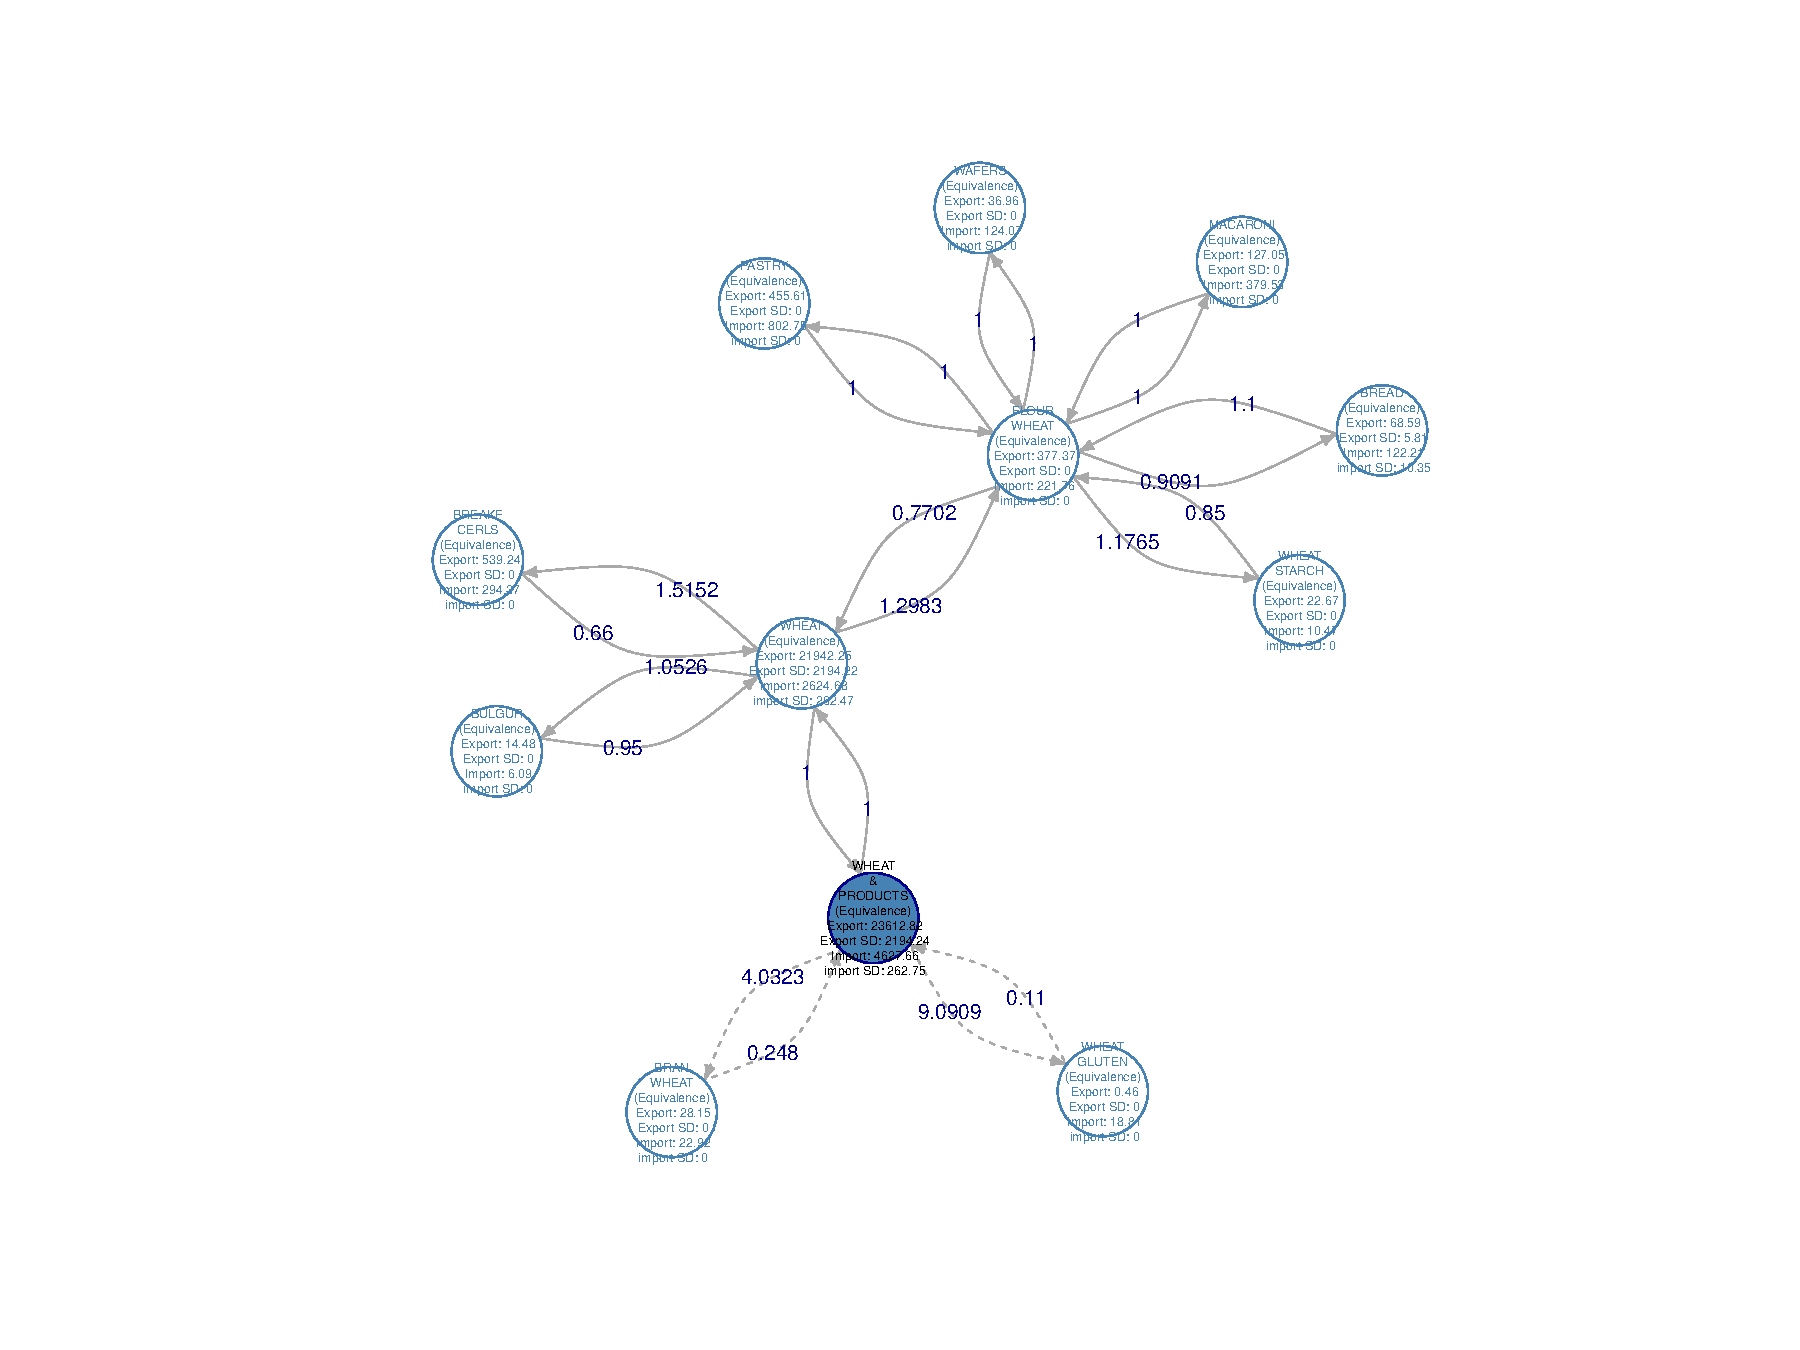
\includegraphics[scale = 0.33]{wheat_usa_2009_distribution_standardized_network.pdf}
  \end{figure}  
}


\frame{
  \frametitle{MCMC Solution}

  We don't have to restrict ourself to distribution with analytical
  mixture, as a matter of fact we can speficy any distribution and
  obtain the mixture via MCMC.

  \vfill
  
  We can model the dependency between extraction rate and calorie at
  the same time, and many other joint probability.

}

\frame{
  \frametitle{MCMC Solution}
  
  Let us assume the following complicated situation:
  \begin{align}
    \text{wheat} &\sim \mathcal{U}\left(E_{a, b}, \sum_{i \in \mathcal{T}} I_{b, a}\right)\nonumber \\
    \text{bread} &\sim \mathcal{U}\left(E_{a, b}, \sum_{i \in \mathcal{T}} I_{b, a}\right)\nonumber \\
    \text{Wheat flour \& Bulgur} &\sim \mathcal{N}(\boldsymbol{\mu}, \boldsymbol{\Sigma}) \nonumber\\
    \text{Pastry} &\sim \Gamma(\alpha, \beta) \nonumber
  \end{align}  
  
  Then the final standardization will be a mixture distribution and
  does not have to be restricted to any standard probability
  distribution.
 
}

\frame{
  \frametitle{Mixture distribution of wheat equivalent}

  \begin{figure}
    \centering
    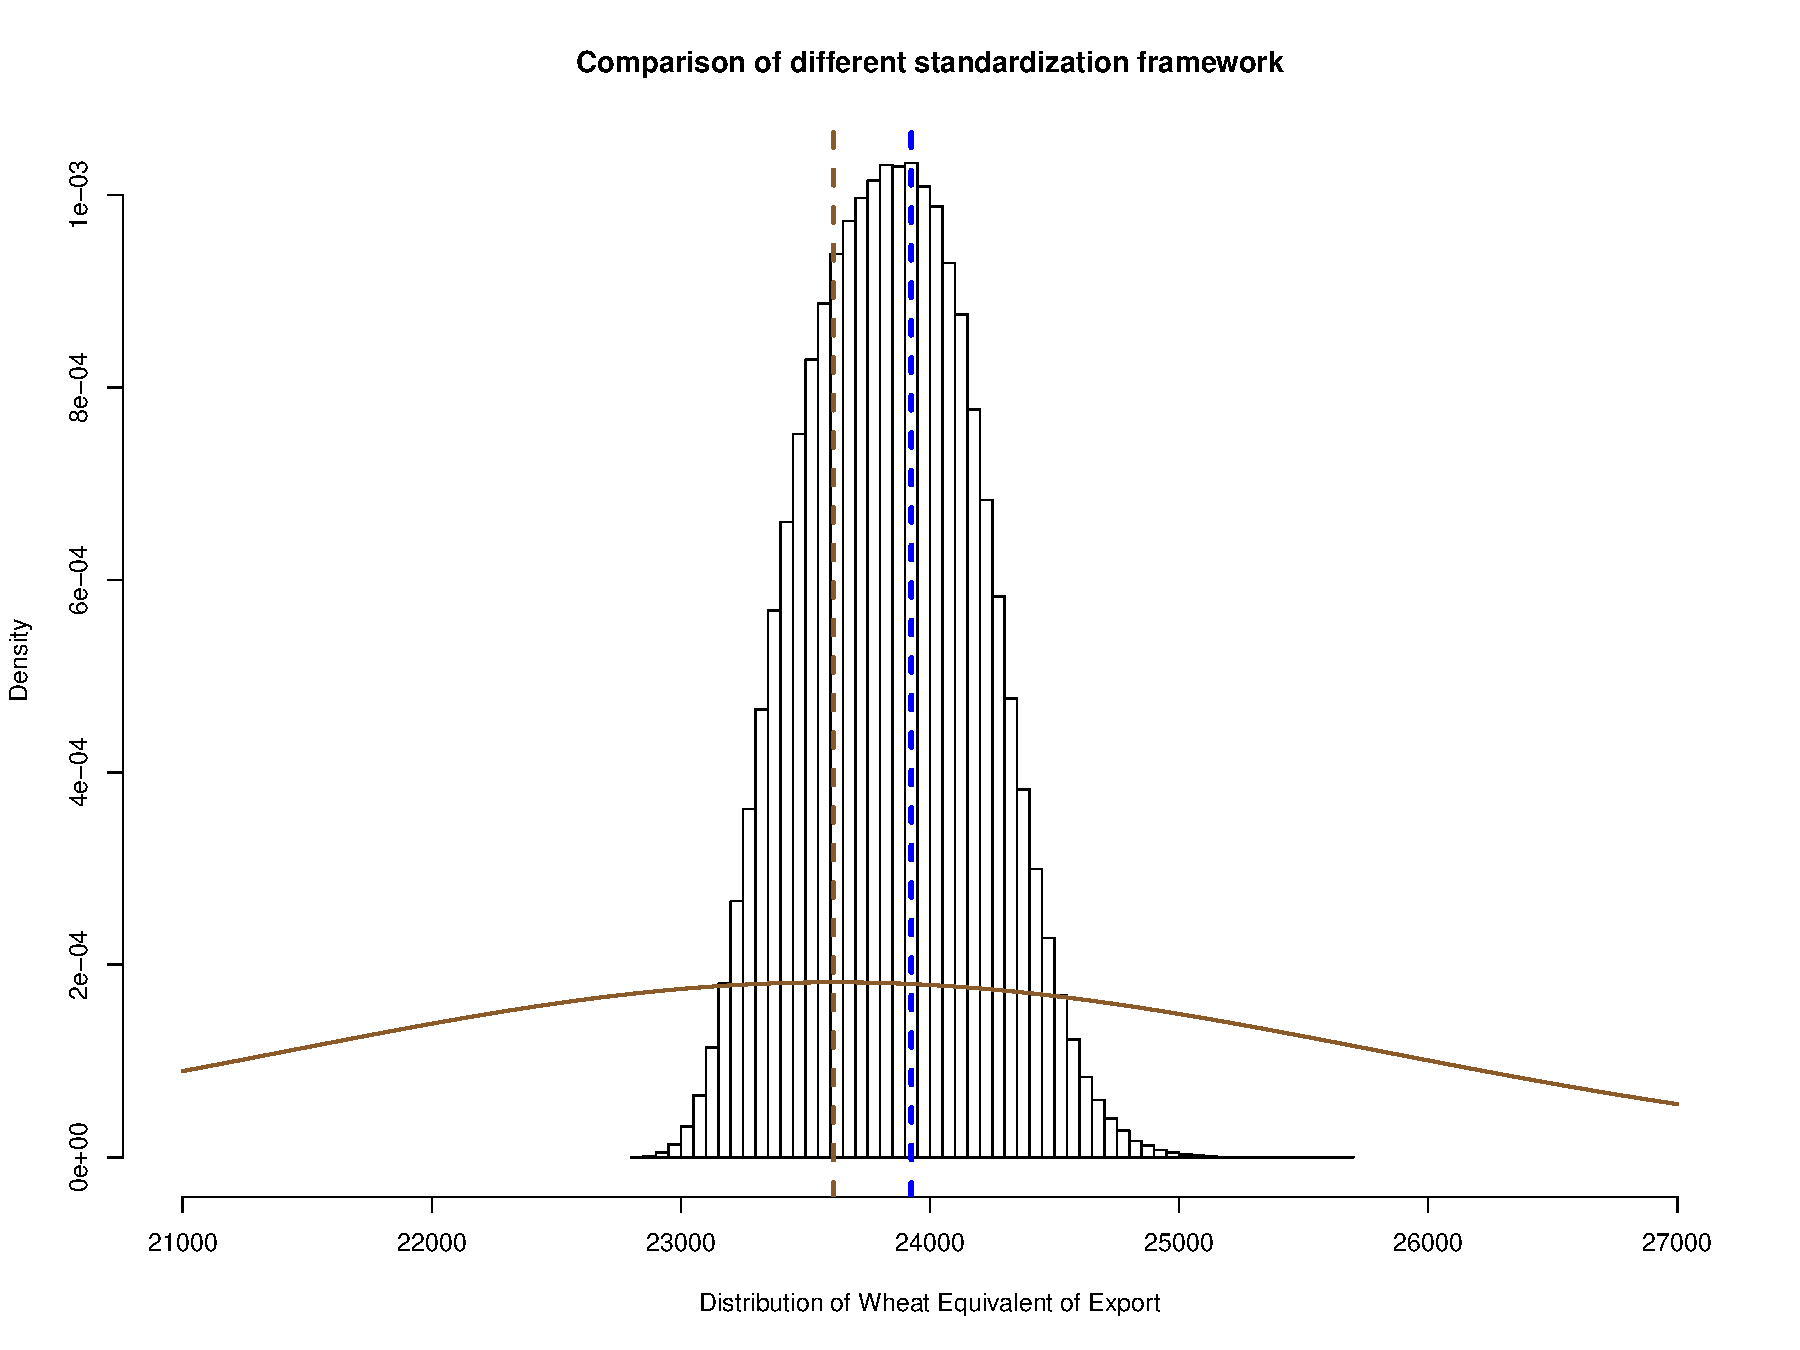
\includegraphics[scale = 0.3]{wheat_mcmc_standardization.pdf}
  \end{figure}    
}

%% \frame{
%%   \frametitle{Bayesian Network Standardization}

%%   Furthermore, we can specify the network as a Bayesian network to
%%   model the dependency in the distributions.

%%   For example, if the extraction rate of wheat flour is 90\% then we
%%   known the wheat flour may contain traces of bran or germ and thus
%%   has a different calorie content.

%% }

\section{Implications}

%% \frame{
%%   \frametitle{Calibration of quantity and calorie}

%%   There may be potentital ways of calibrate the two in a single model.

%% }


\frame{
  \frametitle{Removal of unecessary accounts}
  
  We no longer need a category called statistical discrepancy.

}

%% \frame{
%%   \frametitle{Uncertainty in data collection and estimation can be captured}

%%   Trade discrepancy can be handled naturally, error associated with
%%   model based estimation can be passed on to the balancing
%%   methodology.

%% }




\frame{
  \frametitle{Integration with other FBS methodology}

  Errors in model based estimate can be preserved and passed to future
  analysis and methodology
  
  \vfill
  
  The new standardization also provides a lower level prior
  distribution for the multiway-contingency sampling in the new FBS
  balancing methodology. It give us more insight about the sources of
  the variability and undertainty rather than guess at the aggregated
  level.


}

\frame{
  \frametitle{Bayesian estimate of the Prevalence of Undernourishment}

  The calorie computed from the standardization and ultimately the
  dietary energy supply (DES) is used for the calculation of the
  Prevalence of Undernourishment (PoU). 

  \vfill

  Bayesian methodology can be developed for PoU to reflect our
  uncertainty about food availability and PoU.

}

\section{Further Work}
\frame{
  \frametitle{How to set the distributions?}
  
  Given the large number of commodity, it may be difficult to set the
  distribution for all the elements accross all country for the whole
  system.

  \vfill

  %% It may be possible to estimate the distribution via the use of
  %% maximum entropy to formulate a full objective Bayesian framework,
  %% but also allow the possibility for human intervention.

}


\frame{
  \frametitle{Integration with other methodology}
  
  Despite the flexibility, the integration of the probabilistic
  standardization with other methodology will require careful and
  comprehensive thought for implementation.

  \vfill
  
  \begin{itemize}
    %% \setlength{\itemindent}{0.1in}
    \item MCMC results will not be replicable, at least not to the
      same degree of accuracy.
    \item Passing parameters from different methodology will require
      special classes to handle ditribution or sample.
  \end{itemize}
  
}


%% \begin{frame}[allowframebreaks]
%%   \frametitle{Reference}
%%   \begin{thebibliography}{10}
%%   \end{thebibliography}
%% \end{frame}
  

\end{document}
